\documentclass{beamer}

% xcolor and define colors -------------------------
\usepackage{xcolor}

% https://www.viget.com/articles/color-contrast/
\definecolor{purple}{HTML}{5601A4}
\definecolor{navy}{HTML}{0D3D56}
\definecolor{ruby}{HTML}{9a2515}
\definecolor{alice}{HTML}{107895}
\definecolor{daisy}{HTML}{EBC944}
\definecolor{coral}{HTML}{F26D21}
\definecolor{kelly}{HTML}{829356}
\definecolor{cranberry}{HTML}{E64173}
\definecolor{jet}{HTML}{131516}
\definecolor{asher}{HTML}{555F61}
\definecolor{slate}{HTML}{314F4F}

% Mixtape Sessions
\definecolor{picton-blue}{HTML}{00b7ff}
\definecolor{violet-red}{HTML}{ff3881}
\definecolor{sun}{HTML}{ffaf18}
\definecolor{electric-violet}{HTML}{871EFF}

\newcommand\pictonBlue[1]{{\color{picton-blue}#1}}
\newcommand\sun[1]{{\color{sun}#1}}
\newcommand\electricViolet[1]{{\color{electric-violet}#1}}
\newcommand\violetRed[1]{{\color{violet-red}#1}}

\newcommand\bgPictonBlue[1]{{\colorbox{picton-blue!20!white}{#1}}}
\newcommand\bgSun[1]{{\colorbox{sun!20!white}{#1}}}
\newcommand\bgElectricViolet[1]{{\colorbox{electric-violet!20!white}{#1}}}
\newcommand\bgVioletRed[1]{{\colorbox{violet-red!20!white}{#1}}}

\def\code#1{\texttt{#1}}

% Main theme colors
\definecolor{accent}{HTML}{00b7ff}
\definecolor{accent2}{HTML}{871EFF}
\definecolor{gray100}{HTML}{f3f4f6}
\definecolor{gray800}{HTML}{1F292D}


% Beamer Options -------------------------------------

% Background
\setbeamercolor{background canvas}{bg = white}

% Change text margins
\setbeamersize{text margin left = 15pt, text margin right = 15pt} 

% \alert
\setbeamercolor{alerted text}{fg = accent2}

% Frame title
\setbeamercolor{frametitle}{bg = white, fg = jet}
\setbeamercolor{framesubtitle}{bg = white, fg = accent}
\setbeamerfont{framesubtitle}{size = \small, shape = \itshape}

% Block
\setbeamercolor{block title}{fg = white, bg = accent2}
\setbeamercolor{block body}{fg = gray800, bg = gray100}

% Title page
\setbeamercolor{title}{fg = gray800}
\setbeamercolor{subtitle}{fg = accent}

%% Custom \maketitle and \titlepage
\setbeamertemplate{title page}
{
    %\begin{centering}
        \vspace{20mm}
        {\Large \usebeamerfont{title}\usebeamercolor[fg]{title}\inserttitle}\\
        {\large \itshape \usebeamerfont{subtitle}\usebeamercolor[fg]{subtitle}\insertsubtitle}\\ \vspace{10mm}
        {\insertauthor}\\
        {\color{asher}\small{\insertdate}}\\
    %\end{centering}
}

% Table of Contents
\setbeamercolor{section in toc}{fg = accent!70!jet}
\setbeamercolor{subsection in toc}{fg = jet}

% Button 
\setbeamercolor{button}{bg = accent}

% Remove navigation symbols
\setbeamertemplate{navigation symbols}{}

% Table and Figure captions
\setbeamercolor{caption}{fg=jet!70!white}
\setbeamercolor{caption name}{fg=jet}
\setbeamerfont{caption name}{shape = \itshape}

% Bullet points

%% Fix spacing between items
\let\olditemize=\itemize 
\let\endolditemize=\enditemize 
\renewenvironment{itemize}{\vspace{0.25em}\olditemize \itemsep0.25em}{\endolditemize}

%% Fix left-margins
\settowidth{\leftmargini}{\usebeamertemplate{itemize item}}
\addtolength{\leftmargini}{\labelsep}

%% enumerate item color
\setbeamercolor{enumerate item}{fg = accent}
\setbeamerfont{enumerate item}{size = \small}
\setbeamertemplate{enumerate item}{\insertenumlabel.}

%% itemize
\setbeamercolor{itemize item}{fg = accent!70!white}
\setbeamerfont{itemize item}{size = \small}
\setbeamertemplate{itemize item}[circle]

%% right arrow for subitems
\setbeamercolor{itemize subitem}{fg = accent!60!white}
\setbeamerfont{itemize subitem}{size = \small}
\setbeamertemplate{itemize subitem}{$\rightarrow$}

\setbeamertemplate{itemize subsubitem}[square]
\setbeamercolor{itemize subsubitem}{fg = jet}
\setbeamerfont{itemize subsubitem}{size = \small}








% Links ----------------------------------------------

\usepackage{hyperref}
\hypersetup{
  colorlinks = true,
  linkcolor = accent2,
  filecolor = accent2,
  urlcolor = accent2,
  citecolor = accent2,
}


% Line spacing --------------------------------------
\usepackage{setspace}
\setstretch{1.35}


% \begin{columns} -----------------------------------
\usepackage{multicol}


% Fonts ---------------------------------------------
% Beamer Option to use custom fonts
\usefonttheme{professionalfonts}

% \usepackage[utopia, smallerops, varg]{newtxmath}
% \usepackage{utopia}
\usepackage[sfdefault,light]{roboto}

% Small adjustments to text kerning
\usepackage{microtype}



% Remove annoying over-full box warnings -----------
\vfuzz2pt 
\hfuzz2pt


% Table of Contents with Sections
\setbeamerfont{myTOC}{series=\bfseries, size=\Large}
\AtBeginSection[]{
        \frame{
            \frametitle{Roadmap}
            \tableofcontents[current]   
        }
    }


% Tables -------------------------------------------
% Tables too big
% \begin{adjustbox}{width = 1.2\textwidth, center}
\usepackage{adjustbox}
\usepackage{array}
\usepackage{threeparttable, booktabs, adjustbox}
    
% Fix \input with tables
% \input fails when \\ is at end of external .tex file
\makeatletter
\let\input\@@input
\makeatother

% Tables too narrow
% \begin{tabularx}{\linewidth}{cols}
% col-types: X - center, L - left, R -right
% Relative scale: >{\hsize=.8\hsize}X/L/R
\usepackage{tabularx}
\newcolumntype{L}{>{\raggedright\arraybackslash}X}
\newcolumntype{R}{>{\raggedleft\arraybackslash}X}
\newcolumntype{C}{>{\centering\arraybackslash}X}

% Figures

% \imageframe{img_name} -----------------------------
% from https://github.com/mattjetwell/cousteau
\newcommand{\imageframe}[1]{%
    \begin{frame}[plain]
        \begin{tikzpicture}[remember picture, overlay]
            \node[at = (current page.center), xshift = 0cm] (cover) {%
                \includegraphics[keepaspectratio, width=\paperwidth, height=\paperheight]{#1}
            };
        \end{tikzpicture}
    \end{frame}%
}

% subfigures
\usepackage{subfigure}


% Highlight slide -----------------------------------
% \begin{transitionframe} Text \end{transitionframe}
% from paulgp's beamer tips
\newenvironment{transitionframe}{
    \setbeamercolor{background canvas}{bg=accent!40!black}
    \begin{frame}\color{accent!10!white}\LARGE\centering
}{
    \end{frame}
}


% Table Highlighting --------------------------------
% Create top-left and bottom-right markets in tabular cells with a unique matching id and these commands will outline those cells
\usepackage[beamer,customcolors]{hf-tikz}
\usetikzlibrary{calc}
\usetikzlibrary{fit,shapes.misc}

% To set the hypothesis highlighting boxes red.
\newcommand\marktopleft[1]{%
    \tikz[overlay,remember picture] 
        \node (marker-#1-a) at (0,1.5ex) {};%
}
\newcommand\markbottomright[1]{%
    \tikz[overlay,remember picture] 
        \node (marker-#1-b) at (0,0) {};%
    \tikz[accent!80!jet, ultra thick, overlay, remember picture, inner sep=4pt]
        \node[draw, rectangle, fit=(marker-#1-a.center) (marker-#1-b.center)] {};%
}


% DAGS ----------------------------------------------
\usepackage{tikz}
\usetikzlibrary{shapes,decorations,arrows,calc,arrows.meta,fit,positioning}
% Tikz settings optimized for causal graphs.
\tikzset{
    -Latex,auto,node distance =1 cm and 1 cm,semithick,
    state/.style ={ellipse, draw, minimum width = 0.7 cm},
    point/.style = {circle, draw, inner sep=0.04cm,fill,node contents={}},
    bidirected/.style={Latex-Latex,dashed},
    el/.style = {inner sep=2pt, align=left, sloped}
}


% Beamer tricks -------------------------------------
% Make \pause work in align environments
\makeatletter
\renewrobustcmd{\beamer@@pause}[1][]{%
  \unless\ifmeasuring@%
  \ifblank{#1}%
    {\stepcounter{beamerpauses}}%
    {\setcounter{beamerpauses}{#1}}%
  \onslide<\value{beamerpauses}->\relax%
  \fi%
}
\makeatother




\begin{document}

\imageframe{./lecture_includes/cover_understanding.png}

\section{Where do (Good) Instruments Come From?}

\subsection{True Lotteries}
\begin{frame}{Subtlties of the Validity Condition}
\begin{itemize}
\item To apply IV, we need to make a good case for instrument validity \\ (note we can always check relevance!)\pause{}
\medskip
\item Consider our simple causal model, $Y_i=\alpha+\beta D_i+\varepsilon_i$. Validity $Cov(Z_i,\varepsilon_i)=0$ intuitively requires two distinct assumptions:\smallskip\pause{}
\begin{itemize}
\item \emph{As-good-as-random assignment}: individuals with higher/lower potential earnings face the same distribution of $Z_i$\smallskip
\item \emph{Exclusion}: the ``assignment'' of $Z_i$ only affects $Y_i$ through $D_i$
\end{itemize}
\medskip\pause{}

\item Confusingly, old-school econometrics texts sometimes refer to $Cov(Z_i,\varepsilon_i)=0$ as the ``exclusion restriction''
\smallskip\pause{}

\begin{itemize}
\item More modern IV texts take care to distinguish between these two conceptually distinct requirements... 
\end{itemize}
\end{itemize}
\end{frame}

\begin{frame}{A Valid Instrument}
\begin{center}
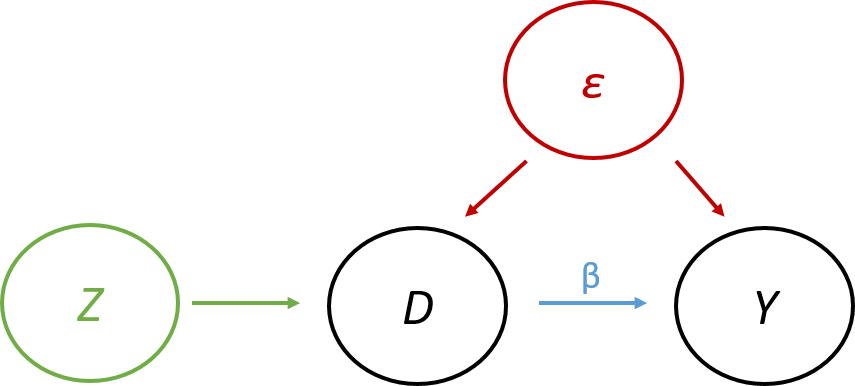
\includegraphics[scale=0.6]{./lecture_includes/dag3.png}
\end{center}
\end{frame}

\begin{frame}{A Violation of As-Good-As-Random Assignment}
\begin{center}
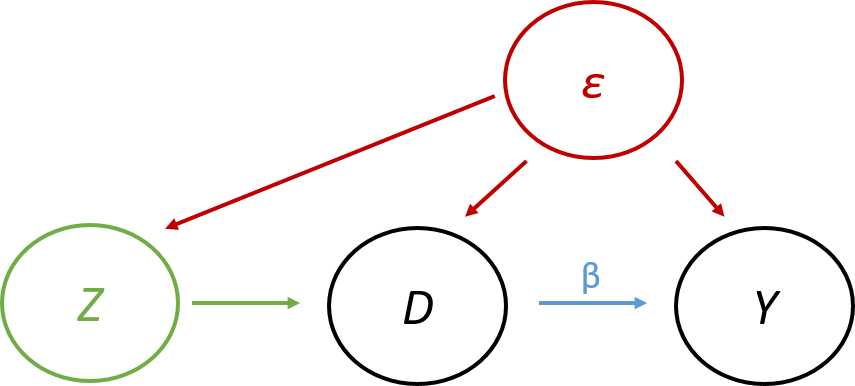
\includegraphics[scale=0.6]{./lecture_includes/dag4.png}
\end{center}
\end{frame}

\begin{frame}{A Violation of Exclusion}
\begin{center}
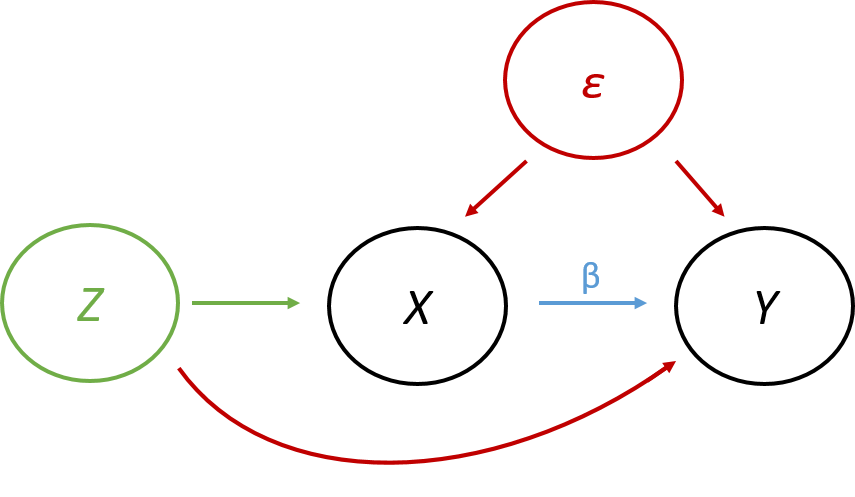
\includegraphics[scale=0.6]{./lecture_includes/dag5.png}
\end{center}
\end{frame}

\begin{frame}{Where do IVs Come From? 1) True Lotteries}
\begin{itemize}
\item One sure-fire way to ensure that a $Z_i$ is as-good-as-randomly assigned is... \pause{} to randomly assign it!\pause{}\smallskip
\begin{itemize}
\item Some of the best IVs come from lotteries, either run by the researcher (e.g. an RCT) or so-called ``natural experiments''
\smallskip
\item We still need to worry about violations of the exclusion restriction
\smallskip
\item Relevance holds when $Z_i$ has some effect on $X_i$
\end{itemize}\pause{}
\medskip

\item ``Gold standard'' IV: a randomized offer to participate in a program, with $X_i$ recording program participation\smallskip
\begin{itemize}
\item Exclusion restriction likely to hold for any $Y_i$, by construction
\smallskip
\item Relevance almost guaranteed (provided people want the program!)
\end{itemize}
\end{itemize}
\end{frame}

\begin{frame}{Example: Charter School Lotteries}
\begin{itemize}
\item Abdulkadiroglu et al. (2016) are interested in whether going to a ``charter'' middle school increases standardized test scores\smallskip
\begin{itemize}
\item Charter students tend to score better, but we worry about selection
\smallskip
\item History of doubting educational inputs, since Coleman (1966)
\end{itemize}
\medskip\pause{}
\item We leverage an institutional feature of charters: \emph{admission lotteries}\smallskip
\begin{itemize}
\item When more kids want to enroll than there are seats, admission offers $Z_i\in\{0,1\}$ are effectively drawn from a hat
\smallskip
\item Offers plausibly only affect later test scores $Y_i$ by changing charter enrollment $D_i\in\{0,1\}$, so are plausibly valid instruments
\smallskip
\item We need to control for lottery fixed effects (``risk sets'') to make $Z_i$ as-good-as-randomly assigned -- more on this soon
\end{itemize}
\medskip\pause{}
\item We study a particular charter (UP Academy), which is ``takeover''\smallskip
\begin{itemize}
\item Two offer IVs: ``immediate'' (on lottery night) and from a waitlist
\end{itemize}
\end{itemize}
\end{frame}

\begin{frame}{Lottery IV Estimates of UP Test Score Effects}

\begin{center}
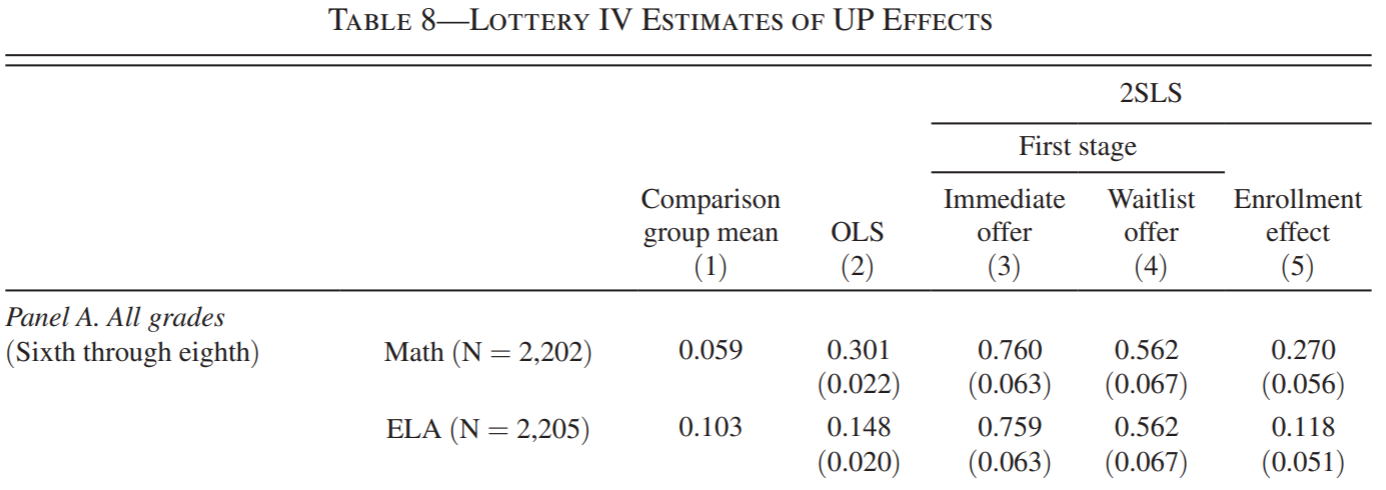
\includegraphics[scale=0.32]{./lecture_includes/charters1.png}
\end{center}

\end{frame}

\subsection{Natural Experiments}
\begin{frame}{Natural Experiments}
\begin{itemize}
\item Without appealing to literal randomization, we may credibly argue $Z_i$ is as-good-as-randomly assigned conditional on some $\mathbf{W}_i$\smallskip
\begin{itemize}
\item Such ``quasi-experiments'' rely on a selection-on-observables argument (for $Z_i$, instead $D_i$)
\smallskip
\item Still worry about exclusion: $Z_i$ cannot affect $Y_i$ except through $D_i$
\end{itemize}\pause{}\medskip
\item Angrist and Krueger (1991) famously estimate labor market returns to schooling with a creative IV: student quarter-of-birth\smallskip
\begin{itemize}
\item Compulsory schooling requirements prevent students from dropping before the day they turn 16 (used to be more binding)
\smallskip
\item Fixed school start dates mean students who drop out at 16 get more or less schooling depending on their birth date\pause{}
\smallskip
\item Quarter-of-birth seems quasi-randomly assigned... is it excludable? Some evidence that older students learn more in each grade...
\end{itemize}
\end{itemize}
\end{frame}


\subsection{Panel Data}
\begin{frame}{Exclusion}
Stuff about Exclusion
\end{frame}

\section{2SLS Mechanics}

\subsection{Just-Identified IV}
\begin{frame}{Just-Identified IV}
Stuff about just-identified IV
\end{frame}

\subsection{Overidentification}
\begin{frame}{Overidentification}
Stuff about overidentification
\end{frame}

\section{Weak and Many Instruments}

\subsection{Weak IV}
\begin{frame}{Weak IV}
Stuff about weak IV
\end{frame}

\subsection{Many IVs}
\begin{frame}{Many IVs}
Stuff about many IVs
\end{frame}

\end{document}
